\section{Sensor systems}
	\label{sec:sensorsystems}
	\subsection{BioHarness}
			The Zephyr Bioharness 3 \cite{bioharness} is a physiolocigal monitoring device, which is attached to a strap on the chest. There are several practical uses for this device.
			\begin{itemize}
				\item Remote patient monitoring. Medical patients who need health care but want to live at home, in combination with ZephyrLIFE \texttrademark \cite{bhpatients}.
				\item Sporters who would like to track their progress.
				\item For coaches to find out who is tired and up for substitution during a match \cite{bhsport}.
				\item In 2010 Chilean mineworkers who were trapped underground were remotedly monitored which resulted in a better rescue order and better health care when the miners were again above ground \cite{chile}.
				\item Researchers who could use the data.
			\end{itemize}

			The device has an internal storage for more than 500 hours logging and the battery's life cycle is up to 35 hours. The device can be connected to a pc with a USB cable, to transfer data and to recharge the battery. The following logs could be produced: general log, summary log, summary and waveform log and the event log. 
			It takes around 1-6 minutes per hour of data to download the log files from the device to a computer \cite{bhdatasheet}. The data is stored in a folder per session (a period from which the device is on till it is turned off) and within the folder different CSV\footnote{CSV stands for Comma-Separated Values and such file can be opend with e.g. Microsoft Excel. Zypher also provides scripts to convert CSV files to Matlab files.} and DaDisp\footnote{``DADiSP scientific computing and data visualization software that combines the power of programming with the simplicity of a spreadsheet'' \cite{dadisp}.} files. The sampling frequency of the CSV files differs from the sampling frequency of the sensors. Most logs are sampled at \SI{1}{\hertz}. The symbol \SI{}{\hertz} stands for hertz and is defined as the number of cycles per second. The price is \$ 472.
		
			The accelerometer measures the physical acceleration of the user in the x-, y- and z-axis and its unit is in $g$. One $g$ is 9.880665 metres per second squared.  The sampling rate is 100 Hz. The range is from $-16g$ to $16g$ for each axis. The acceleration magnitude is $\sqrt{(\Delta X)^2+(\Delta Y)^2+(\Delta Z)^2}$.

			The breathing sensor measures the pressure of the chest to the sensor. If the pressure is above a certain threshold it will count as a breath taken. The breath rate is the amount of breaths taken in a minute. The sampling frequency is 25 Hz and the ranges is from 0 to 120.

			The electrocardiography (ECG) \cite{ECG} sensor measures the electrical activity of the heart. See Figure~\ref{fig:ecg} for a graph of the results an ECG produces. The sampling frequency is 1000 Hz.

			\begin{figure}[h]
				\centering
					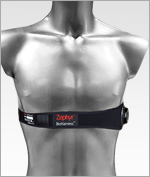
\includegraphics[scale=2.0]{bh.jpg}
					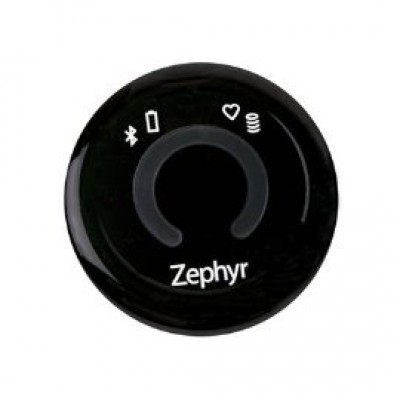
\includegraphics[scale=0.25]{bhclose.jpg}
					
					\caption{The BioHarness.}

			\end{figure}

			\begin{figure}[h]
				\centering
					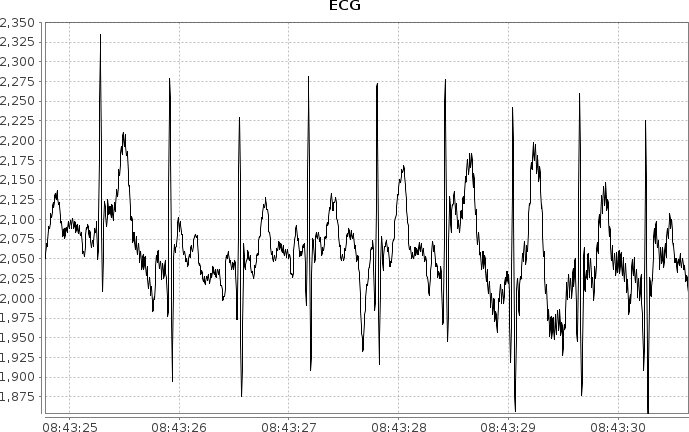
\includegraphics[scale=0.5]{ecg.png}
					
				\caption{A graph of 5 seconds of ECG data.}
				\label{fig:ecg}

			\end{figure}
			
			% R-R: 250 - 1500 ms, 25 Hz

			% heart rate, R-R interval, breathing rate, ECG, postsure, activity, acceleration

			%The data in stored in a csv file and is an 2D array, for every session a csv file. it's resampled to \SI{1}{Hertz}.
		%Timestamp,HR,BR,Temp,Posture,Activity,Acceleration,Battery,BRAmplitude,ECGAmplitude,ECGNoise,XMin,XPeak,YMin,YPeak,ZMin,ZPeak
	\subsection{Beddit}
		%\subsubsection{General}
		The Beddit Sleep Tracker is placed next to a bed and is connected with a sensor between the sheets and the mattress. The makers of Beddit think sleep is important, because a human is sleeping one third of his live. Better sleep results in a better life quality. Why not measure it to help improve our sleep quality? The sensor is about \SI{70}{\centi\metre} long and \SI{4}{\centi\metre} wide, so it is possible it will not cover the whole bed. 
			The price is \EUR{395}.

			The ballistocardiogram (BCG) measures (micro)movements of the body. \cite{beddit}
			BCG is convenient in use, because you will not notice it is measuring, but the disadvantage compared to ECG it is not only measuring cardiac activity, but also body movements, like tossing and turning, which could also be an advantage. \cite{bcg} The sampling frequency is \SI{140}{\hertz}. The devices also measure the room temperature (\SI{}{\celsius}), ambient noise level (\SI{}{\decibel}) and brightness (\SI{}{\lux}), once per 5 minutes \cite{bedditapi}.

			Javascript Object Notation (JSON) is a format to exchange data between different software environments. The data of Beddit is stored in two JSON files per session.

			\begin{figure}[h]
				\centering
					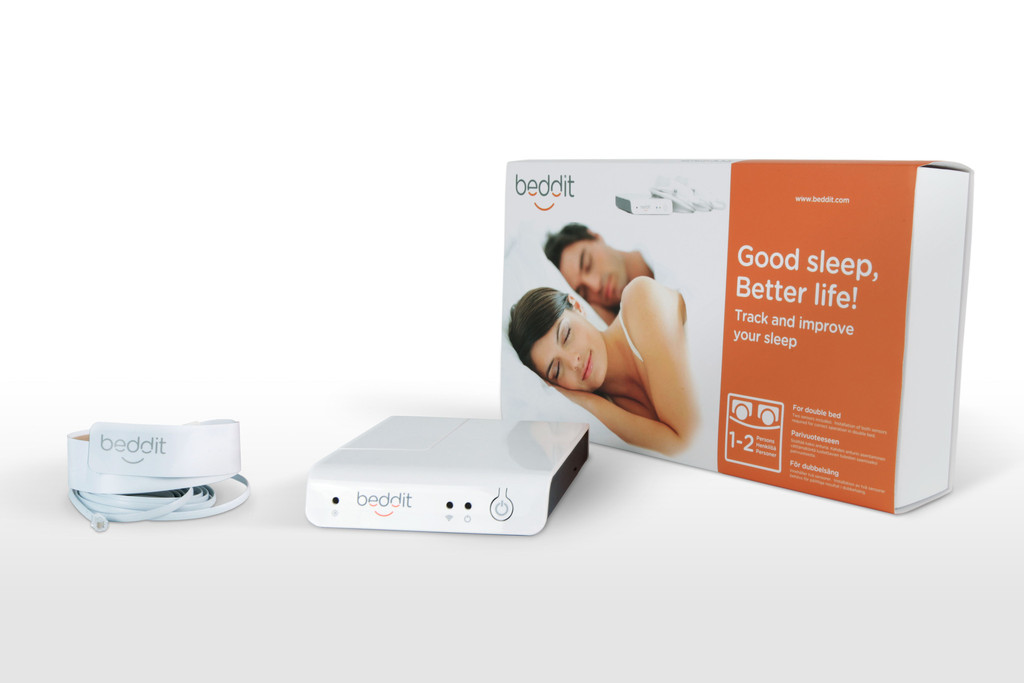
\includegraphics[scale=0.25]{beddit.jpg}
					
					\caption{The Beddit sensor and the device \cite{beddit}.}

			\end{figure}

		%\subsubsection{Description}
		%		Respiration, presence, ihr, actigram, noise, luminosity, temperature, sleep stages, 
		% \subsubsection{Format}
		%	Per day there are two JSON files.
		%	\lstset { 
		%		basicstyle = \footnotesize,
		%		tabsize = 2
		%	}
			%\lstinputlisting[caption=Sleep]{beddit.listing}
			%\lstinputlisting[caption=Results]{beddit2.listing}


	\subsection{Openbeacon}
		%\subsubsection{General}
	RFID stands for Radio-frequency identification and is a technology to communicate wireless between tags. The OpenBeacon Ethernet EasyReader PoE II (called OpenBeacon from now) can receive and send signals with those tags. See Figure~\ref{fig:openbeacon} for a picture of a tag and the device. There are two kind of tags, active and passive ones. Active tags are powered by a battery and can broadcast their signal. Passive tags do not have batteries and are powered by the energy received wireless from the OpenBeacon, but only when they are in range. The tags of the Openbeacon are active tags and can also communicate with each other. The OpenBeacon Ethernet EasyReader PoE II can identify RFID tags and edges between the tags. Each tag has it is own ID and each edge has a power level. It takes the Openbeacon a few seconds to identify the edges. The price of 100 RFID tags is \EUR{1575,75} and the EasyReader costs \EUR{184,87} euro. RFID tags have a lot of applications, like: theft protection on clothing, as access key pas to enter buildings, track and trace of goods while transporting and social experiments \cite{2008arXiv0811.4170B} \cite{socialrfid}. The OpenBeacon produces JSON output.


			\begin{figure}[h]
				\label{fig:openbeacon}
				\centering
					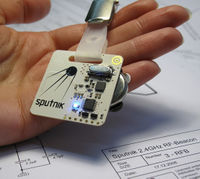
\includegraphics[scale=0.5]{tag.jpg}
					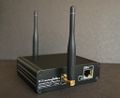
\includegraphics[scale=1.0]{reader.jpg}
					
					\caption{A tag for the OpenBeacon \cite{openbeacon} and the OpenBeacon Reader.}

			\end{figure}

		%\subsubsection{Description}
		%timestamp, tag1, tag2, power level

		%\subsubsection{Format}
		%The data is stored in a MongoDB in the following format:
		%Tags: ID, Timestamp
		%Edges: Timestamp, Tag1, Tag2
